\section{问题一的模型建立与求解}
\subsection{径向热湿传递模型}
将药材近似为半径 $R=0.02\,\mathrm m$、长度 $L=0.25\,\mathrm m$ 的圆柱体。
用 $T(r,t)$ 表示温度（$^\circ\mathrm C$），$C(r,t)$ 表示干基含水率（kg水/kg干物质）。
在预热阶段假设圆柱尺寸不变、周向均匀，忽略端面交换引起的轴向变化，仅求解径向传递。
已有圆柱干燥研究采用导热与水分扩散描述内部温湿场\cite{hussain2003}；本题的物性、初值及交换系数均取自题给附录2，不移用文献样品的经验参数。

依据径向导热与有效扩散关系，建立
\begin{align}
\rho c_p\frac{\partial T}{\partial t}
 &=\frac1r\frac{\partial}{\partial r}\left(rk\frac{\partial T}{\partial r}\right),\label{eq:q1_heat}\\
\frac{\partial C}{\partial t}
 &=\frac1r\frac{\partial}{\partial r}\left[rD(C)\frac{\partial C}{\partial r}\right],
 &D(C)&=7\times10^{-9}\exp\left(-\frac{0.89}{C}\right).\label{eq:q1_moisture}
\end{align}
其中 $\rho=820\,\mathrm{kg/m^3}$、$c_p=2600\,\mathrm{J/(kg\cdot K)}$、
$k=0.36\,\mathrm{W/(m\cdot K)}$，$D$ 的单位为 $\mathrm{m^2/s}$。
初始条件为 $T(r,0)=28$、$C(r,0)=2.55$；中心满足对称条件 $T_r(0,t)=C_r(0,t)=0$。
记烘房温度和水分浓度为 $T_a(t)$、$C_a(t)$，表面采用
\begin{equation}
-kT_r(R,t)=h[T(R,t)-T_a(t)],\qquad
-D(C_s)C_r(R,t)=h_m[C_s-C_a(t)],\label{eq:q1_robin}
\end{equation}
其中 $C_s=C(R,t)$，$h=25\,\mathrm{W/(m^2\cdot K)}$、$h_m=8\times10^{-7}\,\mathrm{m/s}$。
空气含湿量与药材干基含水率的基准不同，此处将题给浓度差及传质系数作为有效经验边界闭合，不将其解释为已测定的吸附平衡关系。
温度方程未显式计入蒸发潜热，其结果适用于所选等效模型。

对附件1中 $0$--$1800\,\mathrm s$ 的31个环境记录采用保形分段三次 Hermite 插值（PCHIP），
逐点保留观测值，不平滑数据。本问温度物性为常数且未引入潜热，温度方程与水分方程分别求解；水分方程始终保留 $D(C)$ 的非线性。

\subsection{有限体积离散与数值检验}
在 $0\le r\le R$ 上设置包含中心和表面的非均匀节点，将相邻节点中点作为控制体边界。
第 $i$ 个环形控制体的径向权重为
\begin{equation}
W_i=\int_{r_{i-1/2}}^{r_{i+1/2}}r\,\mathrm dr
=\frac{r_{i+1/2}^2-r_{i-1/2}^2}{2}.
\end{equation}
以 $F_{i+1/2}=-r_{i+1/2}D_{i+1/2}(C_{i+1}-C_i)/(r_{i+1}-r_i)$
表示向外的径向水分通量，则 $W_i\dot C_i=F_{i-1/2}-F_{i+1/2}$。
面扩散系数取相邻节点系数的调和平均；中心内侧通量为零，表面通量直接由式\eqref{eq:q1_robin}给出。
热传递按同一控制体积分，储热权重为 $\rho c_pW_i$。
该写法通过控制体积分处理中心，不在 $r=0$ 直接计算 $1/r$。

半离散系统采用隐式后向差分公式（BDF）积分。
在表面附近加密网格，同时使题目要求的每隔 $0.1\,\mathrm{cm}$ 输出位置均为计算节点。
比较529、1057和2113个节点，选用2113节点结果。
生产计算相对容差为 $10^{-10}$，温度和含水率绝对容差分别为 $10^{-10}$ 和 $10^{-12}$，最大时间步长为 $0.5\,\mathrm s$；另将容差缩小5倍、最大步长减半，检查时间敏感性。

温度的独立线性参考由分离变量与 Duhamel 叠加构造。
令 $\alpha=k/(\rho c_p)$、$\mathrm{Bi}=hR/k$，特征根满足
$\lambda_nJ_1(\lambda_n)=\mathrm{Bi}J_0(\lambda_n)$，则
\begin{align}
T(r,t)&=T_a(t)-\sum_{n=1}^{\infty}A_nJ_0(\lambda_nr/R)I_n(t),\\
A_n&=\frac{2J_1(\lambda_n)}{\lambda_n[J_0(\lambda_n)^2+J_1(\lambda_n)^2]},
\qquad \dot I_n=-\frac{\alpha\lambda_n^2}{R^2}I_n+\dot T_a(t).
\end{align}
其中 $J_0,J_1$ 为第一类 Bessel 函数，$I_n(0)=T_a(0)-28$。
将截断项数加倍并核对全部输出点变化后，才使用其作为参考。
水分的解析对照仅用于将 $D$ 冻结在初值后的辅助问题，不能代替式\eqref{eq:q1_moisture}的非线性答案。

相邻两层细网格的温度、含水率最大差分别为 $5.90\times10^{-7}$ 和 $4.56\times10^{-6}$，均小于预设的 $2\times10^{-5}$ 数值目标。
表1、表2在空间与时间加密后均保持四位小数不变；完整输出中仍有接近舍入分界的数值发生末位变化，不能据此声称所有单元格的第四位均已冻结。
温度与独立参考的最大差为 $2.15\times10^{-7}$。
对连续数值解的表面通量按 PCHIP 区间自适应积分，热、湿累计收支的相对残差分别为 $2.05\times10^{-9}$ 和 $2.43\times10^{-11}$。
以上检验针对离散与积分误差，不代表经验参数及真实药材预测具有同样精度。

\subsection{预热阶段的温度与含水率分布}

\begin{table}[H]
\centering
\caption{30分钟内药材温度（$^\circ\mathrm C$）}\label{tab:q1_T}
\small
\begin{tabular}{rrrrrr}
\toprule
时间/s & \multicolumn{5}{c}{到中心的距离/cm}\\
\cmidrule(lr){2-6}
 & 0 & 0.5 & 1.0 & 1.5 & 2.0\\
\midrule
100 & 28.0000 & 28.0003 & 28.0038 & 28.0319 & 28.1795 \\
300 & 28.0406 & 28.0634 & 28.1513 & 28.3673 & 28.8486 \\
600 & 28.4533 & 28.5361 & 28.8039 & 29.3155 & 30.1641 \\
900 & 29.3243 & 29.4583 & 29.8757 & 30.6164 & 31.7295 \\
1200 & 30.5429 & 30.7099 & 31.2225 & 32.1130 & 33.4295 \\
1500 & 31.9960 & 32.1871 & 32.7667 & 33.7476 & 35.1211 \\
1800 & 33.5758 & 33.7724 & 34.3642 & 35.3626 & 36.7879 \\
\bottomrule
\end{tabular}
\end{table}

\begin{table}[H]
\centering
\caption{30分钟内药材干基含水率（kg/kg）}\label{tab:q1_C}
\small
\begin{tabular}{rrrrrr}
\toprule
时间/s & \multicolumn{5}{c}{到中心的距离/cm}\\
\cmidrule(lr){2-6}
 & 0 & 0.5 & 1.0 & 1.5 & 2.0\\
\midrule
100 & 2.5500 & 2.5500 & 2.5500 & 2.5500 & 2.2470 \\
300 & 2.5500 & 2.5500 & 2.5500 & 2.5492 & 2.0508 \\
600 & 2.5500 & 2.5500 & 2.5500 & 2.5353 & 1.8770 \\
900 & 2.5500 & 2.5500 & 2.5497 & 2.5045 & 1.7547 \\
1200 & 2.5500 & 2.5500 & 2.5482 & 2.4646 & 1.6586 \\
1500 & 2.5500 & 2.5499 & 2.5445 & 2.4206 & 1.5787 \\
1800 & 2.5500 & 2.5497 & 2.5383 & 2.3755 & 1.5102 \\
\bottomrule
\end{tabular}
\end{table}
在1800 s时，烘房温度为 $41.513\,^\circ\mathrm C$。
药材表面温度为 $36.7879\,^\circ\mathrm C$，中心温度为 $33.5758\,^\circ\mathrm C$。
表面先响应环境升温，热量向内传递形成径向梯度。
表面干基含水率降至 $1.5102$，中心仍为 $2.549992$（四位显示为 $2.5500$），说明短时失水主要集中在外层。
中心四位显示不变并不意味着中心完全没有失水。

\begin{figure}[H]
\centering
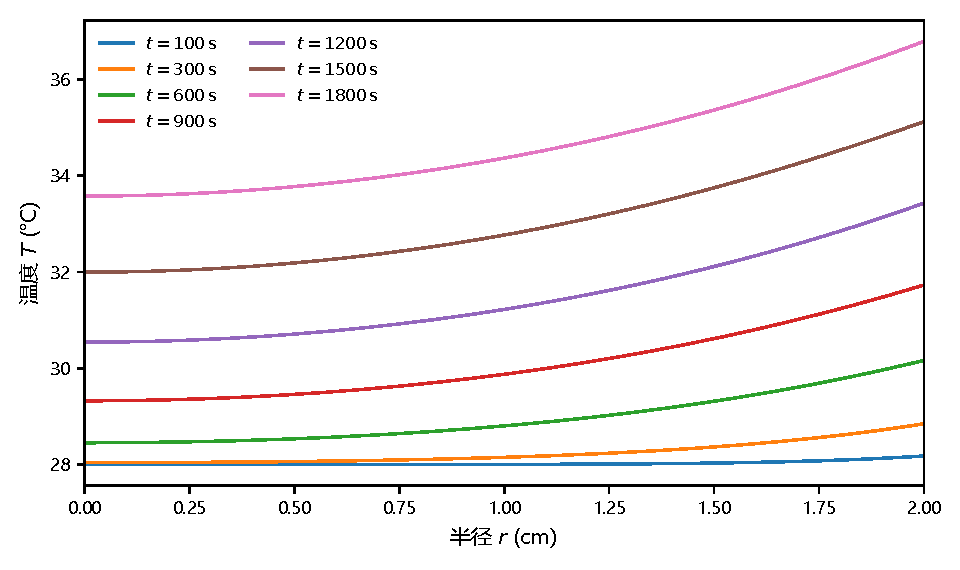
\includegraphics[width=.70\textwidth]{../figures/q1_T_profiles.pdf}
\caption{预热阶段不同时间的径向温度分布}\label{fig:q1_T}
\end{figure}

\begin{figure}[H]
\centering
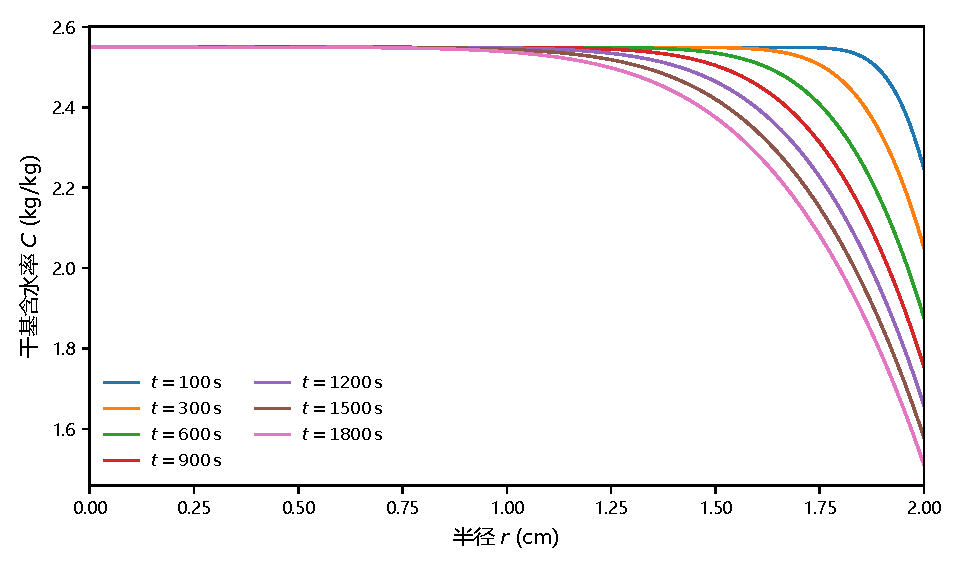
\includegraphics[width=.70\textwidth]{../figures/q1_C_profiles.pdf}
\caption{预热阶段不同时间的径向干基含水率分布}\label{fig:q1_C}
\end{figure}
含水率下降使局部扩散系数减小，外层失水与内部补水形成动态耦合。
题目要求的逐秒温度和含水率按每隔 $0.1\,\mathrm{cm}$ 输出至 \texttt{result1.xlsx}，显示保留四位小数，计算及后续核查使用未舍入值。
忽略潜热和端面交换是本模型的主要局限；上述数值检验不消除这些物理近似。
